\subsection{Import und Verarbeitung des FEM-Gitters}
In diesem Abschnitt wird kurz der Import und die Verarbeitung des im vorherigen Kapitel erstellten FEM-Gitters beschrieben. Dabei wird genauer auf die Methodik zur korrekten Interpretation der Randbedingungen eingegangen. So erfordert zum Beispiel die Berechnung des Elementgleichungssystems ein Kurvenintegral entlang des neumannschen Randes, wobei sich diese aus mehreren Dreiecksseiten zusammensetzt. Somit ist es zwingend notwendig aus dem generierten Gitter herauszulesen welche Seite oder Seiten der entsprechenden Elemente am neumannschen Rand liegen.

\subsubsection{Import des Gitters}
Wie schon zuvor erwähnt unterstützt benötigt die Software eine Gitterdatei der Version 2. Dabei handelt es sich um ASCII-codierte Dateien mit mindestens folgenden Informationen:

\begin{itemize}
	\item Das Format der Datei im Abschnitt \textit{\$MeshFormat\$}. Sie Software unterstützt nur Dateien der Version 2.2.0.8
	
	\item Informationen über die 'Physical Groups' der Problemgeometrie im Abschnitt \textit{\$Physical Names\$}. Dabei gibt der erste Eintrag des Abschnitts die Anzahl der 'Physica Groups' an. Jeder weitere Eintrag steht für eine 'Physical Group' definiert durch jeweils drei Parameter:
	\begin{enumerate}
		\item Dimension der 'Physical Group'. 1: 1-dimensional (Kurve), 2: 2-dimensional (Fläche)
		\item ID. Jede Gruppe bekommt eine positive Ganzzahl zur eindeutigen Identifikation zugewiesen.
		\item Name. Jener Name der in Gmsh der Gruppe zugewiesen wurde.
	\end{enumerate}

	\item Daten der Elementkonten des Gitters im Abschnitt \textit{\$Nodes\$}. Der erste Eintrag gibt wieder die Anzahl der Knoten an, jeder weitere Eintrag steht für einen Knoten, wobei die erste Zahl eine positive Ganzzahl zur eindeutigen Identifizierung des Knotens darstellt. Die weiteren drei Einträge sind Gleitkommazahlen für die x-, y- und z-Koordinaten.
	
	\item Die Definitionen der finiten Elemente im Abschnitt \textit{\$Elements\$}. Der erste Eintrag gibt wieder Anzahl der Elemente an, und jeder weiter Zeile definiert ein Element nach dem folgenden Schema:
	\begin{enumerate}
		\item ID. Eine positive Ganzzahl zur eindeutigen Identifikation des Elements.
		\item Typ des Elements. Gmsh kennt viele verschiedene Elementtypen. Für eine vollständige Liste sei auf die Dokumentation von Gmsh verwiesen (\cite{gmsh_website}). Da sie Software dreieckige finite Elemente bis zur Ordnung 3 unterstützt sind hier folgende Einträge möglich:
		\begin{itemize}
			\item 2: 2-knotige lineare Linie/Kurve
			\item 3: 3-knotiges lineares Dreieckselement
			\item 8: 3-knotige quadratische Line/Kurve
			\item 9: 6-knotiges quadratisches Dreieckselement
			\item 26: 4-knotige kubische Linie/Kurve
			\item 21: 10-knotiges kubisches Dreieckselement
		\end{itemize}
		\textbf{Anmerkung:} In Zukunft könnten weitere Elementtypen unterstützt werden.
		\item Der nächste Eintrag gibt die Anzahl der 'Physical Tags' an. Auch hier sei zu deren genauen Bedeutung auf die Dokumentation von Gmsh verwiesen.\cite{gmsh_website}. Standardmäßig ist der erste Eintrag danach die ID der 'Physical Group' der das Element angehört. Alle Weiteren 'Tags' werden nicht benötigt.
		\item 'Physical Tage'. Siehe vorheriger Punkt.
		\item IDs der Elementknoten. Je nach Elementtyp (siehe oben) finden sich nun die IDs der Knoten welche das Element definieren. Dabei ist zu beachten dass Gmsh die Knoten anders als das FEM-Tool definiert. Hierbei sei auf die Gmsh Dokumentation, Abschnitt 9.2 verwiesen. Die Definition welche das FEM-Tool verwendet findet sich in diesem Dokument unter Abschnitt \ref{sec:finite_elements_and_shape_functions}. Es ist also ein Umordnen der Knoten notwendig, was jedoch von der Software automatisch beim Import durchgeführt wird.
	\end{enumerate}
\end{itemize}

Eine Beispielhafte Gitterdatei zu dem in Abbildung \ref{fig:neumann_boundary_assignment} gezeigten Beispiel findet sich in Code \ref{fig:example_mesh_file}.


\subsubsection{Verarbeitung der Gitterinformation}
Nach erfolgreichem Import der Gitterinformation ist als letzter Schritt or der eigentlichen Lösung nun notwendig die Randbedingungen des Problems, sowie Materialeigenschaften und weitere Informationen wie zum Beispiel Quellen (freie Raumladungen etc.) den einzelnen Elementen zuzuordnen. Hierbei kommen die bei der Erstellung der Geometrie definierten 'Physical Groups' zum Tragen. \newline

Wie im vorherigen Abschnitt erwähnt, ist jedes finite Element einer solchen Gruppe zugeteilt. Für die hier betrachteten zweidimensionalen Probleme können zwei Arten von \textit{Physical Groups} definiert werden: Kurven (\textit{Physical Curves}) und Flächen (\textit{Physical Surfaces}). Erstere beschreiben die dirichletschen und neumannschen Randbedingungen und Ihnen sind somit nur eindimensionale Element zugeordnet. Letztere beschreiben die Materialen des Problemgebietes sowie dessen Quellen. Daher sind solchen Gruppen nur zweidimensionale Elemente zugeordnet.\newline

Folgende Parameter müssen nun jedem Element zugeordnet werden:
\begin{itemize}
	\item Knoten am dirichletschen Rand: Das Potential des entsprechenden Elementknotens ist bereits vorgegeben, was bei der Berechnung des Elementgleichungssystems entsprechend berücksichtigt werden muss.
	\item Knoten und Seiten am neumannschen Rand: Wie in (\ref{eq:right_side_e_static}) ersichtlich erfordert die Berechnung von $r_j$ ein Integral über die neumannsche Randfläche, welche im zweidimensionalen Fall zu einem Kurvenintegral entartet. Dabei ist es wichtig zu wissen welche Dreiecksseite am neumannschen Rand liegt.
	\item Materialeigenschaften im Element: Wie in \ref{eq:k_ij_e_static} ersichtlich ist es notwendig $\epsilon_x$ und $\epsilon_y$ für jedes Element zu kennen. Die Deklaration von $\epsilon_x$ und $\epsilon_y$ erfolgt in einem separaten File, welches in Abschnitt ... genauer behandelt wird. Die Zuordnung zum entsprechenden Element erweist sich als trivial da jeder Elementdefinition die ID der entsprechenden 2D \text{Physical Group} beiliegt.
	\item Analog zu den Materialeigenschaften verhält es sich mit den Quellen innerhalb eines Elements. Die Quellen kommen z.B. bei der Berechnung von (\ref{eq:right_side_e_static}) als Parameter $\rho$ zum Tragen. Auch hier erweist sich die Zuordnung wieder als trivial.
\end{itemize}

Die Zuordnung der Knoten und Dreiecksseiten an den Rändern des Problems wird im folgenden Kapitel beschrieben.

\subsubsection{Zuordnung der Knoten am dirichletschen- und Dreiecksseiten am neumannschen Rand}
Wie bereits oben erwähnt ist eine direkte Zuordnung der Dreieckselemente am dirichletschen und neumannschen Rand nicht möglich. Vielmehr muss ein Umweg über die eindimensionalen Elemente gegangen werden. Die angewandten Algorithmen werden im Folgenden beschrieben: \newline

\textbf{Knoten am dirichletschen Rand:}
\begin{enumerate}
	\item Man ermittle alle Elementknoten am gewählten Rand aus den dem Rand zugeordneten Kurvenelementen. Da die Definition der Kurvenelemente in der Gitterdatei bereits die ID der entsprechenden \textit{Physical Group} enthält ist diese Aufgabe trivial.
	\item Man suche nun alle Dreieckselemente die die vorher ermittelten Knoten beinhalten und speichere diese Zuordnung samt Randwerte für die entsprechenden Knoten.
\end{enumerate}

\textbf{Dreiecksseiten am neumannschen Rand:}
\begin{enumerate}
	\item Man wende den gleichen Algorithmus wie oben an.
	\item Man ermittle die Dreiecksseite am neumannschen Rand durch Vergleich der Rand- und Elementknoten:\newline
	Je nach Elementtype ist eine Dreiecksseite durch 2, 3 oder 4 Knoten definiert. Siehe dazu Abschnitt \ref{sec:finite_elements_and_shape_functions}. Liegt ein Dreieckselement am neumannschen Rand, so stimmen alle Knoten einer oder mehrerer Seiten mit den Knoten am Rand überein. Hierbei ist zu erwähnen dass auch bei mehr als 2 Knoten pro Seite immer nur eine ganze Seite am Rand liegen kann! \newline
	Wie aus (\ref{eq:right_side_e_static}) bekannt muss ein Kurvenintegral entlang der entsprechenden Dreiecksseite am neumannschen Rand durchgeführt werden. Aufgrund der Verwendung von isoparametrischen finiten Elementen sind im lokalen Koordinatensystem nur drei verschiedene Kurvenintegrale möglich, was eine statische Zuordnung eines Kurvenintegrals zu jeder Seite ermöglicht. Zu diesem Zweck wird jeder Dreiecksseite eine Nummer zugewiesen von welcher ausgehend ein bestimmtes Kurvenintegral berechnet wird. Die Zuordnung lautet wie folgt:
	\begin{itemize}
		\item Die Dreiecksseite auf der $\xi$-Achse sei definiert als \textit{Seite 1}.
		\item Die Dreiecksseite auf der $\eta$-Achse sei definiert als \textit{Seite 2}.
		\item Die verbleibende Seite sei definiert als \textit{Seite 3}
	\end{itemize}
	\begin{figure}[H]
		\begin{center}
			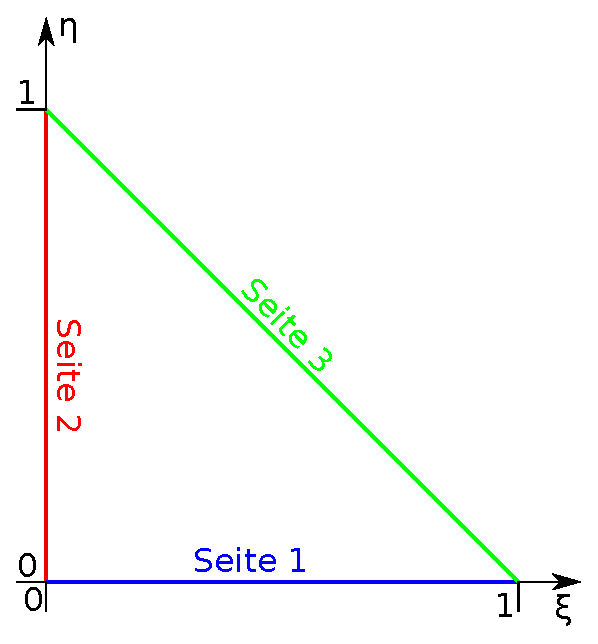
\includegraphics[scale=0.65]{pics/triangle_side_assignment.eps}
		\end{center}
		\caption{Zuordnung der Dreiecksseiten}
		\label{fig:triangle_side_assignment}
	\end{figure}
	\item Zu guter Letzt ordne man noch den Dreiecksseiten am Rand den Wert der Randbedingung (in (\ref{eq:right_side_e_static}) der Parameter $\sigma$) zu.
\end{enumerate}

Um die in diesem Abschnitt gezeigten Zusammenhänge zu verdeutlichen, wird die Zuordnung der Dreiecksseiten zum neumannschen Rand anhand des in Abbildung \ref{fig:neumann_boundary_assignment} gezeigten Beispiels verdeutlicht. Eine Beispielhafte Gitterdatei ist in Code \ref{fig:example_mesh_file} gezeigt.

\lstinputlisting[frame=single, backgroundcolor=\color{lightgray}, basicstyle=\ttfamily\footnotesize, caption = {Exemplarische Gitterdatei}, label={fig:example_mesh_file}, captionpos=b ]{neumann_boundary_assignment_example_mesh_file.txt}

\begin{figure}[htbp]
	\begin{minipage}[t]{0.45\textwidth}
	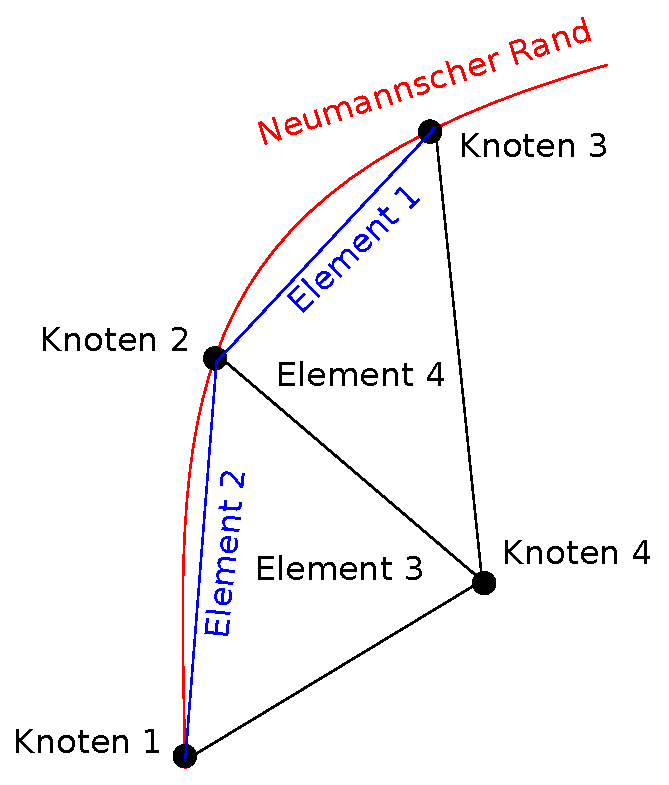
\includegraphics[scale=0.65]{pics/neumann_boundary_assignment.eps}
	\caption{Zuordnung der Dreiecksseiten}
	\label{fig:neumann_boundary_assignment}
	\end{minipage}
	\hfill
	\begin{minipage}[t]{0.45\textwidth}
	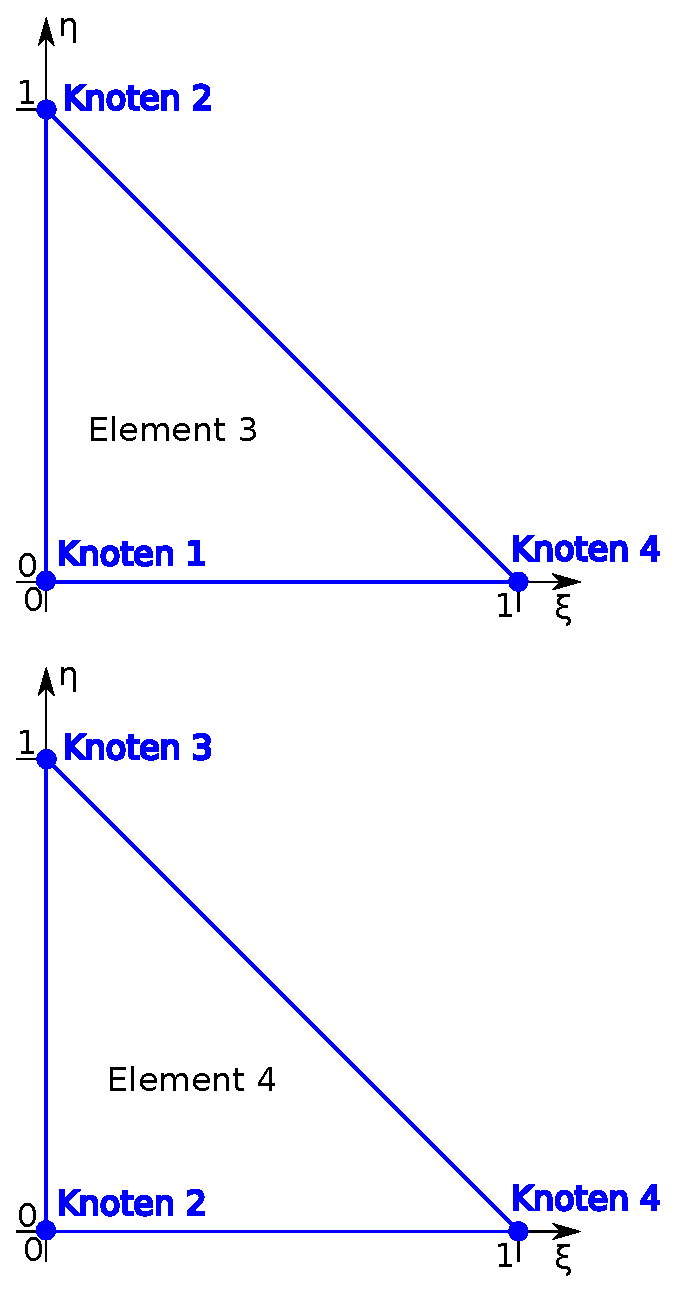
\includegraphics[scale=0.5]{pics/neumann_boundary_assignment_elements_3_4.eps}
	\caption{Elemente 3 und 4 im lokalen Koordinatensystem}
	\label{fig:neumann_boundary_assignment_elements_3_4}
	\end{minipage}	
\end{figure}	

Wie aus Code \ref{fig:example_mesh_file} ersichtlich, setzt sich die Geometrie aus 4 Knoten und 4 Elementen zusammen. Abbildung \ref{fig:neumann_boundary_assignment_elements_3_4} zeigt die Dreieckselemente 3 und 4 in ihrem lokalen Koordinatensystem. 

Wie mit Hilfe von Abbildung \ref{fig:triangle_side_assignment} zu erkennen ist, liegt Element 3 mit Seite 1, und Element 4 mit Seite 2 am neumannschen Rand. Der oben beschrieben Algorithmus wird nun auf dieses Beispiel angewandt um dessen Funktion zu erklären.\newline
\begin{enumerate}
	\item Die Elemente 1 und 2 sind, wie aus Code \ref{fig:example_mesh_file} ersichtlich der \textit{Physical grup} 1 zugeteilt. (Vierter Eintrag in den beiden Elementdefinitionen). Somit ist nun bekannt dass die Knoten 1, 2 und 3 am neumannschen Rand liegen.
	\item Die Knoten 1 und 2 von Element 3 stimmen mit den Knoten am neumannschen Rand überein. Zudem definieren sie die Dreiecksseite 1, über welche in weiterer Folge integriert werden muss. Selbiges lässt sich für Seite 2 von Element 4 durchführen.
\end{enumerate}
